\section{Loading Conditions}
As with any off road vehicle, it is always difficult to predict loading conditions as there is an infinite amount of scenarios due to the varying environment and terrain, however it can usually be generalized to a few simple, yet appropriate cases. Also, it is important for one to remind themselves what the vehicle is being designed for. Although it is an off-road vehicle, it is not designed for extreme conditions or dangerous scenarios. It's the same logic for someone who owns an economical car; they wouldn't be taking this vehicle into the bush through deep mud or rough terrain as it will most likely end up with broken parts. In this case, the robot is to be operated in a normal mining environment where the environment conditions are assumed to be a regular mining road built from crushed, roughly fist sized rock, and a max ramp grade of 20\% or incline of 11.3 degrees. Driving forward up a ramp and a skid steer turn on a ramp were then evaluated. As one could imagine, the skid steer motion when the robot is balancing on two, opposite diagonal wheels resulted in the highest forces, therefore these were used for analysis. With the weight distribution of the coupled wheels being 40/60, the 60\% wheel is used for analysis and its design is to be duplicated to the other wheel. The resulting forces are summarized in     
\\
 ***INSERT TABLE***
\\
It should be noted that only a static analysis was conducted for this project due to slow operating speeds. With a top speed of 3 km/h, the forces due to dynamic loading would only differentiate slightly. To compensate for this, a larger factor of safety was desired for each component. Given an adequate time line, one could conduct a full dynamic simulation to obtain more accurate results and confirm that the design to follow is indeed adequate for the imposed loading conditions. 

\section{Belt Drive}
\subsection{Description}
Synchronous belt drive systems are said to be efficient, reliable, virtually maintenance free and are supposed to outlast any comparable chain drive system. The system used on this vehicle consists of a Gates PowerGrip GT3 belt which is rated for high torque transmission at variable speeds while the sprockets and accompanying bushings were supplied by Martin Sprocket for cost saving reasons.

\subsection{Design Constraints and Functional Requirements}
The overall width of belts and sprockets proved to be a considerable constraint in itself. While there was a specific width required to ensure power transmission without failure, this same width also hindered the design of the drive box as it would result in a thicker and bulkier design. The engineers at Gates were consulted regarding optimization of belt width and sprocket diameters. After a couple weeks of back and forth by email, it was decided that a 30mm wide belt would be best suited.

Next constraint proved to be the diameters of the sprockets as there was an overall size constraint of the drive box. It should also be noted that larger diameters lead to a substantial increase in weight and cost. Therefore finding the happy-medium between required diameter for belt life, overall size, weight and cost was a challenge. There was also the ratio between diameters of the driving sprocket and idlers that needed to remain constant. This ratio, determined by required output speeds and torque transmission, was found to be 1.6.

The position of the idler was also a challenge due to dimensional constraints imposed by the location of the small and large sprockets and ensuring sufficient wrap angle on the driving sprocket. A constraint that wasn’t discovered until part sourcing began was the availability of the sprocket diameters and material selection for these. This proved to be the biggest constraint to overcome since all of those mentioned above also came into play with this constraint.

The goal of the belt drive is to have an efficient and reliable power transmission method that requires minimal maintenance and is easy to assemble and disassemble. Lower operating costs, a dry running drive box and reducing the need for a well sealed drive box are criteria that benefited the design.

\subsection{Analysis and Design}
For the design of the belt system, calculations were done following the design procedure in the Gates PowerGrip GT3 Design Manual and results were verified using the Gates Design IQ software. Using a maximum torque output from the motors of 156 N-m (at 1.2 HP) with an output speed of 60 rpm, a required belt width of 30mm was calculated both by hand and using the software with sprockets having an acceptable size of 72 teeth for the large sprocket and 44 for the small sprocket. A triple check was conducted by the engineers at Gates. They were provided all the details mentioned above and conducted their separate analysis using different software to confirm the results. 

It is important to mention that the belt system will be alternating from clockwise rotation to counterclockwise rotation. This was discussed with the engineers at Gates and they confirmed that since a robust slotted idler is being used, the change between slack and tight side shouldn’t be an issue for this system.
\section{Wheel Shaft Assembly}\label{sec:wheel_shaft_assembly}
The wheel shaft assembly consists of a combination of parts such as bearings, seals and structural members. The assembly needed to be compact, cost efficient and easy to assemble with manufacturability in mind. %With the shaft being the main supporting component connecting the wheels to the drive box, much strength analysis has been conducted for it with varied materials and profiles. The rim mount which boasts the wheel onto the shaft also needed to be an elegant solution that provided self centering fastening. Taper roller bearings were also needed to handle the large axial forces induced by the skid steer motions. In order to house the bearings close to the drivebox, a bearing housing was designed in such a way that limits the flex in the shaft. To run a dry drivebox, radial seals were added to either side of the bearings to contain the grease, but also help limit contamination from the outside environment.

\begin{figure}[h]\centering
	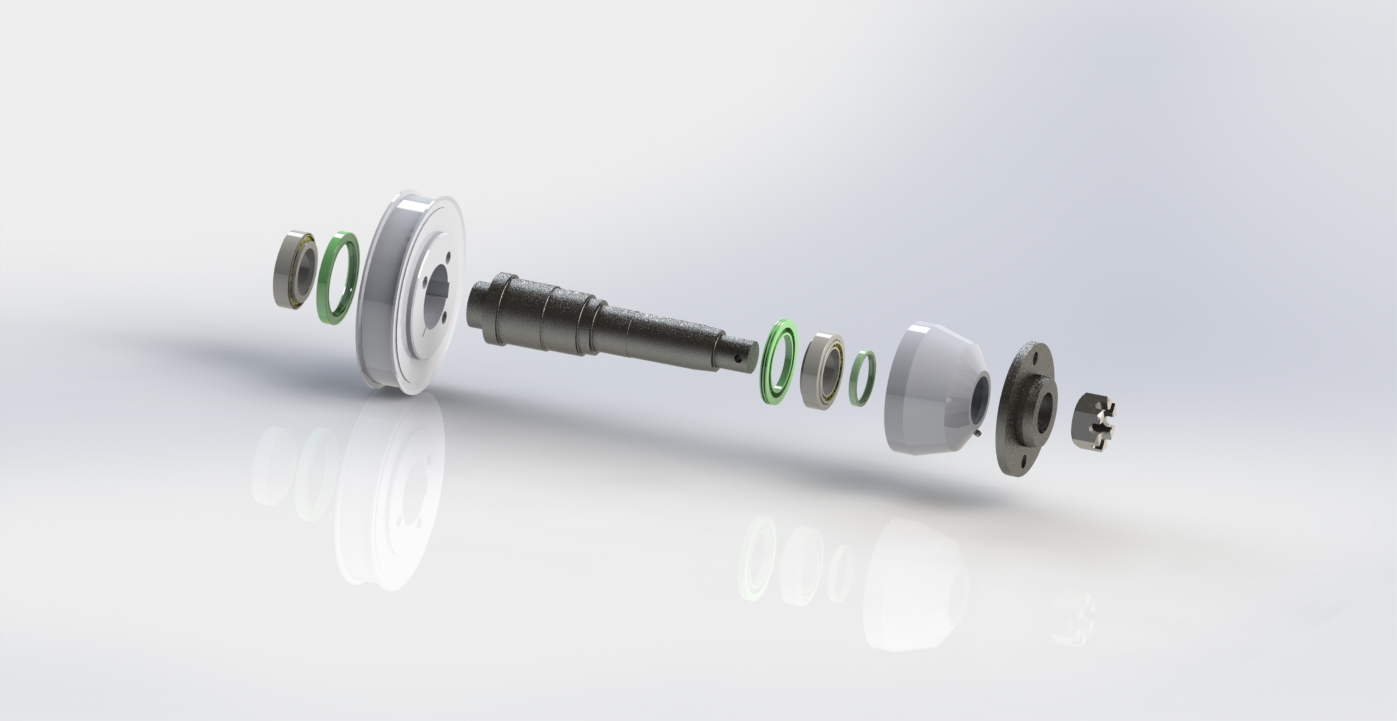
\includegraphics[width=.7\linewidth]{images/explode_wheel_assembly.jpg}
	\caption{Exploded view of wheel shaft assembly.}
	\label{fig:wheel_explode}
\end{figure}

\begin{figure}[h]\centering
	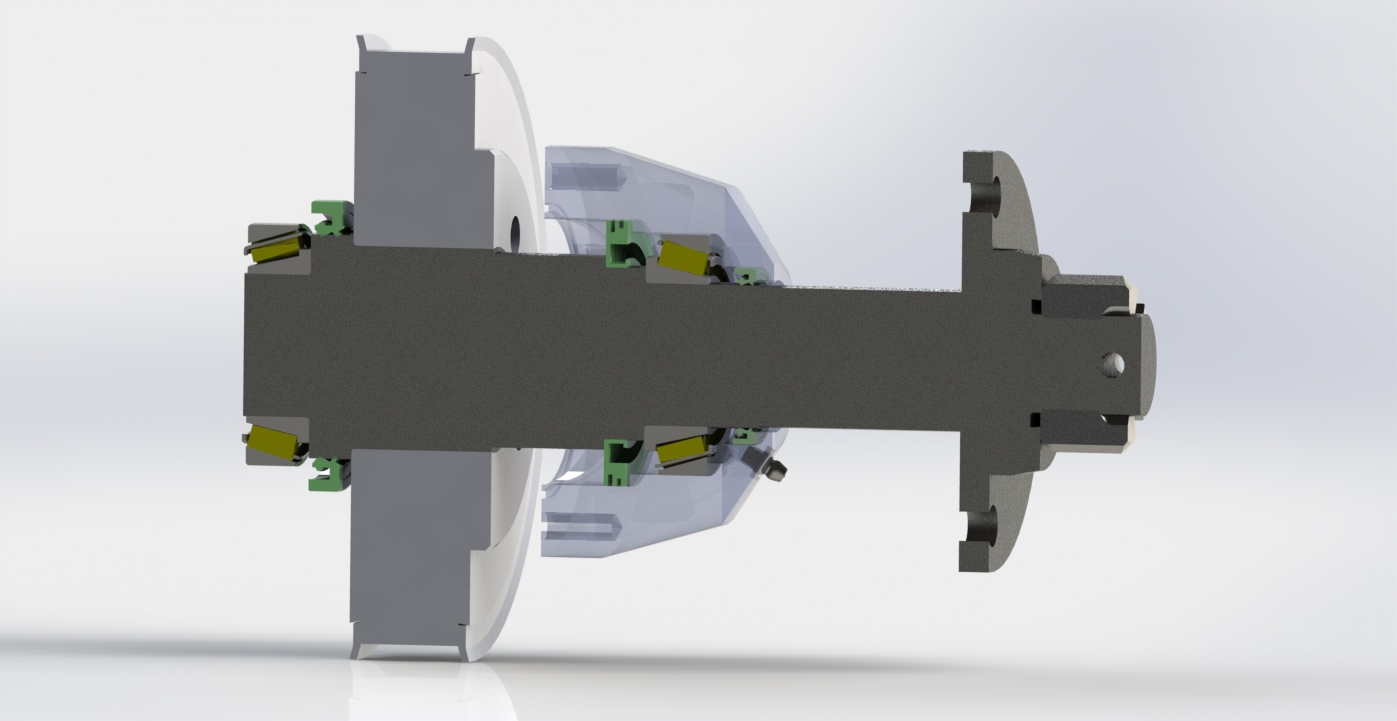
\includegraphics[width=.7\linewidth]{images/wheel_shaft_section.jpg}
	\caption{Section view of wheel shaft assembly.}
	\label{fig:wheel_section}
\end{figure}

\begin{table}[htbp]
	\centering
	\caption{Component details for wheel shaft assembly.}
	\begin{tabular}{| lll |} \hline
		Component & Material & Product Number \\ \hline
		Wheel Shaft & 4340 Steel (Q/T @ 650\degree C) & - \\
		Housing & 6061 Aluminum & - \\
		Rim Mount & 1045 Steel & - \\
		Taper Roller Bearing & - & 32009 X/Q \\
		Large Seal & - & 68x90x10 DL \\
		Medium Seal & - & 2129B \\
		Small Seal & - & 45x55x7 DL \\
		1.25" Castle Nut & Steel & - \\ \hline
	\end{tabular}
	\label{tab:design_spec}
\end{table}


\subsection{Design Constraints and Functional Requirements}
\subsubsection{Wheel Shaft}
The combination of the weight of the vehicle and the forces imposed by the skid steer amounted to large values, thus requiring a strong and durable shaft that experienced minimal flex. Also to consider was the offset imposed by the centered rims on the tires. Clearance between the tires and drive box needed to be large enough to prevent any contact between the two and this in turn increased the overall length of the shaft,and also increasing the large cantilever loading. The shoulders and step diameters on the shaft also needed to match the available sizing of bearings, seals and bushings. It was advised by Penguin ASI that the shafts be made of 4340 steel that is quenched and tempered at 650\degree C for availability, machinability and for company standards reasons.

\subsubsection{Wheel Bearings}
The bearings for this application needed to withstand the large axial forces due to the aggressive skid steer motions and still handle the weight of the vehicle. Size was also an important consideration as larger bearings would directly increased the size of other components such as bearing housings.

\subsubsection{Front Bearing Housing}
The front bearing housing had many factors affecting its design. It needed to house the taper roller bearings that were mounted onto the shaft. In addition, an o-ring groove needed to be added to meet the sealing requirements and two radial seals needed to be added on each side of the bearing. It also needed to be quick and easy to machine. 

\subsubsection{Rear Bearing Housing}
The rear bearing housing serves the same purpose as the front one. It must support the loads applied as well as retained the bearing and provide adequate sealing by means of an o-ring. It must also accommodate a radial seal for the rear bearing and must be a slim as possible to prevent any contact between its back edge and the body shell of the unit under extreme loading conditions.

\subsubsection{Rim Mount}
The rim mount needed to feature a self centering system for ease of installation. Manufacturability was also an important consideration as splines could be costly, while a taper design is cheap and quick. The component also need to withstand all the imposed forces and be easy to replicate for future units. Using in stock materials was also an added bonus for the client.

\subsubsection{Shaft Seals}
Two different style of seals were needed for the proposed method of assembly and shaft layout. The front-interior seal needed shaft mounted, meaning it would be pressed onto the shaft and would seal against the housing while the two outer ones were pressed into their housings and sealed against the shaft. All seals needed to be economical, durable and standard size for availability reasons. Penguin ASI also recommended using seals covered with a nitrile rubber coating for optimal sealing and to meet company standards.

%\subsection{Functional Requirements}
\subsection{Analysis and Design}
\subsubsection{Wheel Shaft}
First step of the design was to set up the shaft layout. Since the belt design had already been done, the dimensions and style of bushings for the sprockets were already known. A certain width was then set aside for bearing width and rim mount location was predetermined to be at the very end of the shaft. The centered rims also required a minimum distance between the drivebox panel and tire. Giving these conditions, a preliminary shaft layout was made for use in the FBD calculations.

Given the previously mentioned loading conditions and general shaft layout, a Matlab script was created to calculate the reaction forces throughout the shaft and generate moment diagrams. A second Matlab script was created to calculate the minimum shaft diameters based the DE Goodman method using previously calculated moments, material properties and shaft features such as keys, fillets and shoulder sizes.

The results obtained from the Matlab script were unreasonably large, however many machine design books state that the DE Goodman is simply a conservative estimate, therefore further finite element analysis using software was conducted. The static simulation resulted in reduced, but more acceptable diameters. 
~\ref {tab:shaft_calc}

\begin{table}[htbp]
	\centering
	\caption{Summary of forces acting on the wheel shaft.}
	\begin{tabular}{| llll |} \hline
		Name & Variable & Value & Unit \\
		Radial Force at wheel & F\textsubscript{ar} & 7600.00 & N \\
		Tangential Force at wheel & F\textsubscript{at} & 546.80 & N \\
		Radial Force at outside bearing & F\textsubscript{br} & 18950.00 & N \\
		Tangential Force at outside bearing & F\textsubscript{bt} & 2333.00 & N \\
		Radial Force at sprocket & F\textsubscript{cr} & 1470.00 & N \\
		Tangential Force at sprocket & F\textsubscript{ct} & 4007.00 & N \\
		Radial Force at inner bearing & F\textsubscript{dr} & 9900.00 & N \\
		Tangential Force at inner bearing & F\textsubscript{dt} & 2220.00 & N \\
		Skid Force & F\textsubscript{skid} & 2476.00 & N \\
		Moment Skid & M\textsubscript{skid} & 566.00 & N \\
		Moment Weight & M\textsubscript{weight} & 48.00 & N \\ \hline
	\end{tabular}
	\label{tab:shaft_calc}
\end{table}

\begin{figure}[h]\centering
	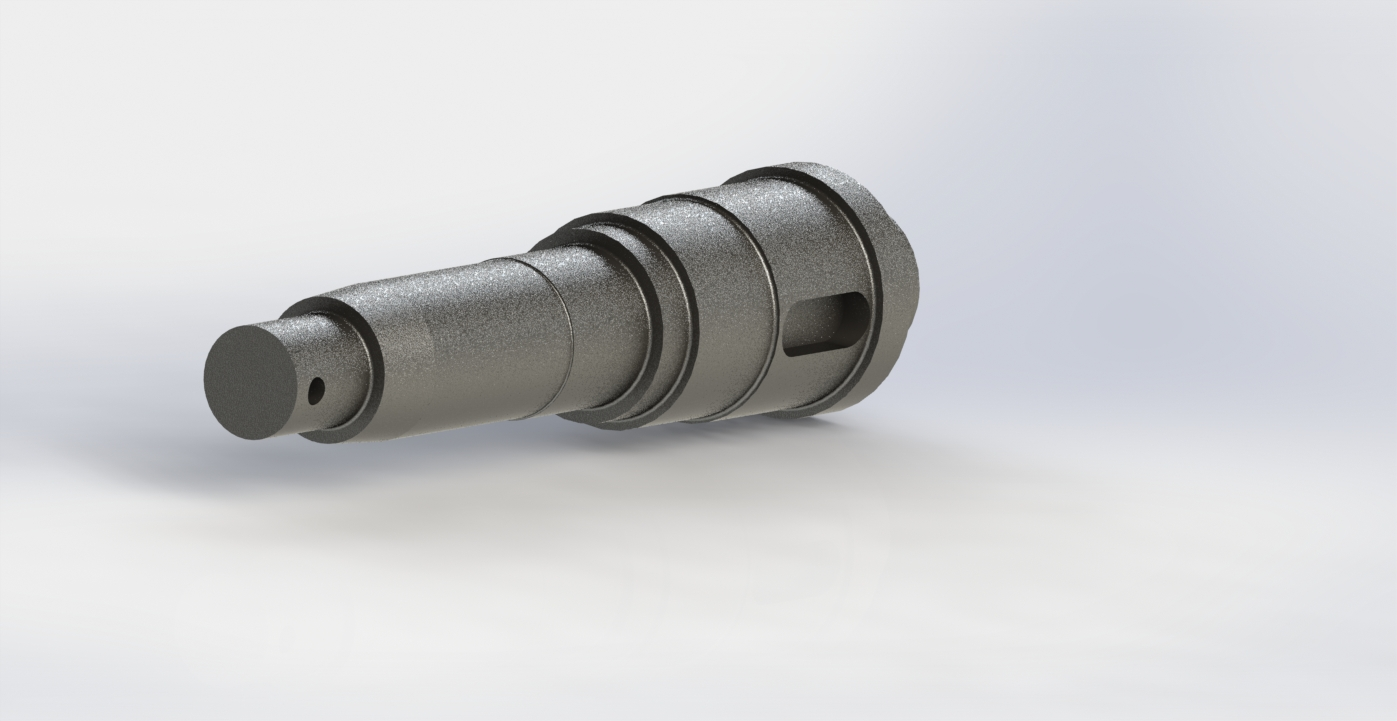
\includegraphics[width=.7\linewidth]{dom/shaft_iso_rndr.jpg}
	\caption{Wheel Shaft}
	\label{fig:wheel_shaft}
\end{figure}

\subsubsection{Wheel Bearings}
Taper roller bearings were selected for their superior axial loading capabilities while still having decent radial loading ratings when compared to other tradition radial bearings. Size for size, these bearings were still competitive as well. Once bearing type was selected, the bearing selection procedure outlined in the SKF Bearing Manual was followed in order to find the optimal bearing for the task. Based on the reaction forces calculated for the wheel shaft and its diameter, properly sized bearings were selected. A proper assessment also included bearing life calculations and taking into consideration the added axial forces by the taper roller bearings. Since the wheel shaft is essentially a cantilever beam, the bearing sizes were quite large and two separate bearings were required. One on the front and another on the back size. For compatibility, interchangeability and availability reasons, both bearings were selected to be identical even though the rear one doesn't see nearly as much loading.

Please refer to Section ~\ref{ws_bearing} for detailed work on bearing selection. See bearing calculations in Figure ~\ref{bearing_calc} in Appendix for a detailed outline of the SKF bearing selection process.

\subsubsection{Shaft Seals}
Two type of shaft seals were required for the proposed shaft layout. The two outermost seals are housing mounted seals. These are the most common type of radial seals and offered the largest selection. Knowing the shaft dimensions from bearing selection and shaft diameters, all that needed to be selected is which style of shaft seal to chose. A conventional seal with a rubber nitrile coating was recommended by the professionals at Penguin ASI. As for the second type of seal, the selection wasn't so obvious. This second seal was to be a shaft mounted seal, however selection for these proved to be very limited. Only metric sizes were available and there we large variations in diameters. Choosing the closest one to the minimum diameter calculated that would fit between the bearing and sprocket left only one option, however this SKF seal still came with the preferred nitrile rubber coating.

Please refer to the wheel shaft BOM for detailed part numbers of shaft seals.

\subsubsection{Front Bearing Housings}
There were many constraints to the front bearing housing and with the seals selected, and bearing dimensions known, the design of this part was fairly straight forward. The goal to utilize in-stock material also determined that 5 inch, 6061 aluminum would be used. Once the design was complete, a check of bolt and thread strength was conducted as well as an FEA of the component under the loading conditions obtained during the wheel shaft calculations. An o-ring groove was also added to provide adequate sealing for the drivebox.

\begin{figure}[h]\centering
	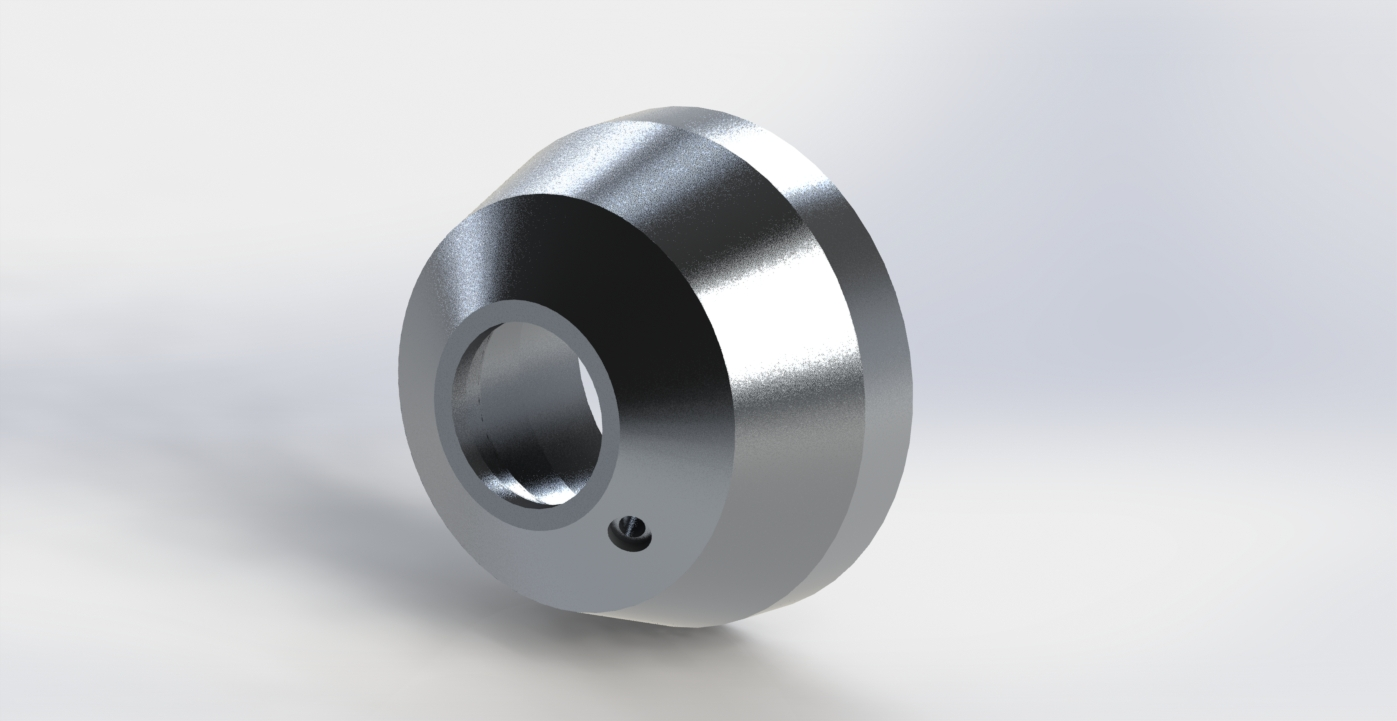
\includegraphics[width=.7\linewidth]{dom/hub_iso_rndr.jpg}
	\caption{Bearing Housing}
	\label{fig:housing}
\end{figure}

Please refer to FEA section of the report for details strength analysis of bearing housing.

\subsubsection{Rear Bearing Housing}
The rear bearing housing was also a straight forward design due to the imposed design constraints. For the same reasons as the front bearing housing, 5 inch 6061 round stock was used and a quick verification of bolt and thread strength was conducted. An o-ring groove was also added for sealing purposes.

The final design of this component varied slightly from the initial one. The outer bore was reduced to increase the outer strength of the unit and for better and quick manufacturability. The depth dimensions didn't change, only the outer diameter did. The new design also meant getting rid of the nuts on the back side of the unit as the new design incorporated the thread inside the components, which also simplified the assembly.

Please refer to the FEA Appendix for more details of rear bearing housing design.

\subsubsection{Rim Mount}
The rim mounts from the previous robot were still in good condition and only needed minor modifications for them to meet the requirements of the new design. Modifications included a change to the bolt pattern and boring out the mounting hole onto the shaft. After some calculations, it was determined that a standard taper hole design of 4.18\degree would be strong enough to resist the rotation moments at the wheels and it would mate perfectly with the taper of the wheel shaft for proper mounting. The taper also has the added benefit of self centering, which is crucial for the design of vehicles to prevent unwanted vibrations due to misalignments and poor performance.

\begin{figure}[h]\centering
	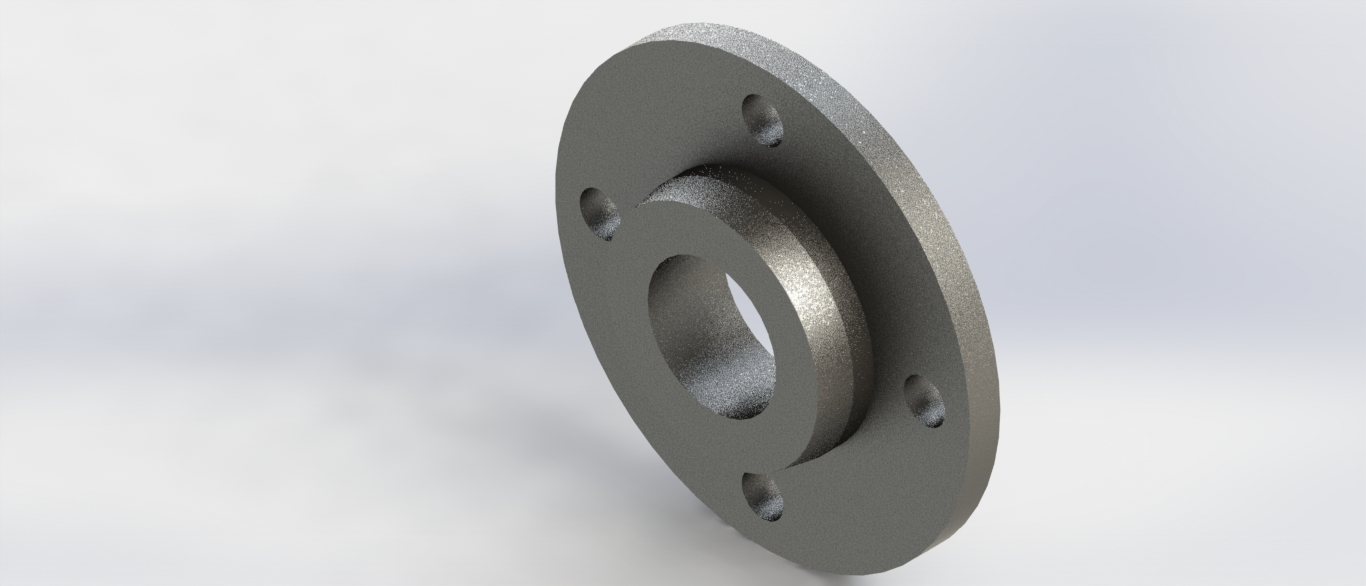
\includegraphics[width=.7\linewidth]{dom/rim_mount_iso_rndr.jpg}
	\caption{Rim Mount}
	\label{fig:rim_mount}
\end{figure}
 

Please refer to Figure ~\ref{taper_calc} for detailed taper strength calculations.

\subsection{Pivot and Travel Limiter}
\subsubsection{Description}

The minimum required shaft diameter was calculated using two iterations of DE Goodman shaft design theory. The second iteration took into account more realistic stress concentrations allowing for the reduction in required shaft diameter. The shaft layout and loading assumptions are illustrated in Figure 24 forces at the ends representing the radial forces applied from the taper roller bearings and the force at the middle being the resultant force of the sprocket determined from the Gates Design IQ software. Bearing calculations were performed according to the procedure outlined in the SKF bearing design manual for taper roller bearings. It is important to note that the free body diagram in Figure 24 only represents the radial component of the force from the taper roller bearing, and axial forces not shown were also taken into consideration. Design constraints and requirements are outlined in Table 18.  

\subsubsection{Design Constraints}

\subsubsection{Functional Requirements}

\subsubsection{Alternate Solution}

\subsubsection{Analysis and Design}

The finite element analysis report for all three revisions of the output shaft can be found in Appendix A.  The revisions 0 and 2 can be seen in the Figure 25 and Figure 26 below. In revision 0 the stresses experienced at the end of the output shaft actually exceed the yield strength of the 4340 steel. The changes between the two shaft layouts are significantly different since the first revision was designed to mount radial bearings onto and the final revision now has a taper roller bearing on each end of the sprocket. Seals are also located on both sides of the taper roller bearing to provide a seal. The stresses experienced in the final revision are greatly reduced and do not exceed the yield strength of the material selected. Fillets were also added to reduce the stress concentrations at the shoulders of the different diameters on the shaft.
\section{Drive Shaft Assembly}
The drive shaft is located between the reduction shaft and the drive box. It is designed to transmit the torque from the reduction shaft to the driving sprocket located within the exterior drive box. The shaft is coupled to the reduction shaft with a flexible coupling and runs the inside of the pivot. There is a key for both ends of the flexible coupling and a set screw on the reduction shaft end. A snap ring was added to the output shaft on the coupling end to allow proper placement of the coupling along the shaft, since the set screw was not reachable once mounted in the pivot. With the pivot being over built to reduce as much deflection as possible at this point it allowed for the output shaft to experience minimal bending moments under loading. The output shaft consists of a bushing for the sprocket, a 3/16" key slot on the reduction end, 3/8" key slot at the sprocket bushing, two taper roller bearings which were located in the cap and the other in the pivot itself and two shaft mounted seals. Figure~\ref{fig:output_shaft} shows the output shaft with the taper roller bearings mounted, shaft seals mounted and the groove for the snap ring at the end that has the flexible coupling attached. The output shafts were manufactured from 1045 steel which was suggested by Penguin ASI since spare material was available in the facility.
\begin{figure}[htbp]
	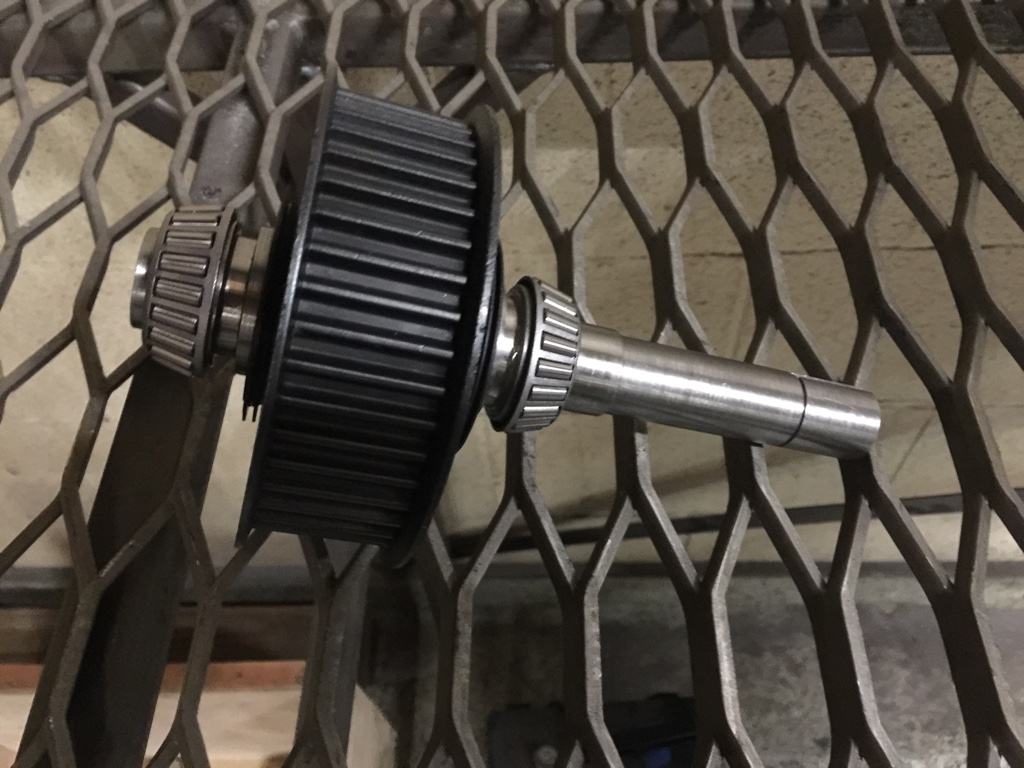
\includegraphics[width=\linewidth]{images/drive_shaft_assembly_bld.jpg}
	\caption{Assembly of output shaft with bearings, seals and sprocket mounted.}
	\label{fig:output_shaft}
\end{figure}
\subsection{Design Constraints and Functional Requirements}
The design of the output shaft had a length constrained to the distances between the reduction shaft and the end of the exterior drive box. It was required to transmit the torques and withstand the radial forces that can be seen in Table~\ref{tab:output_shaft_specs}.   

\subsection{Analysis and Design}
Using the DE-Goodman equation the minimum diameter of the output shaft was able to be calculated after two iterations. The minimum shaft diameter ended up being 20 mm and the bearings were selected using the SKF manual to select the proper taper roller bearings for the loading conditions that can be seen in Figure~\ref{fig:fb_output_shaft}. The free body diagram for the shaft is only the end that contains the two taper roller bearings and the bushing for the sprocket since the coupling end is assumed to be rigid. The finite element analysis for the output shaft can be seen in the Appendix~\ref{sec:drive_shaft_fea}.
\begin{figure}[H]
	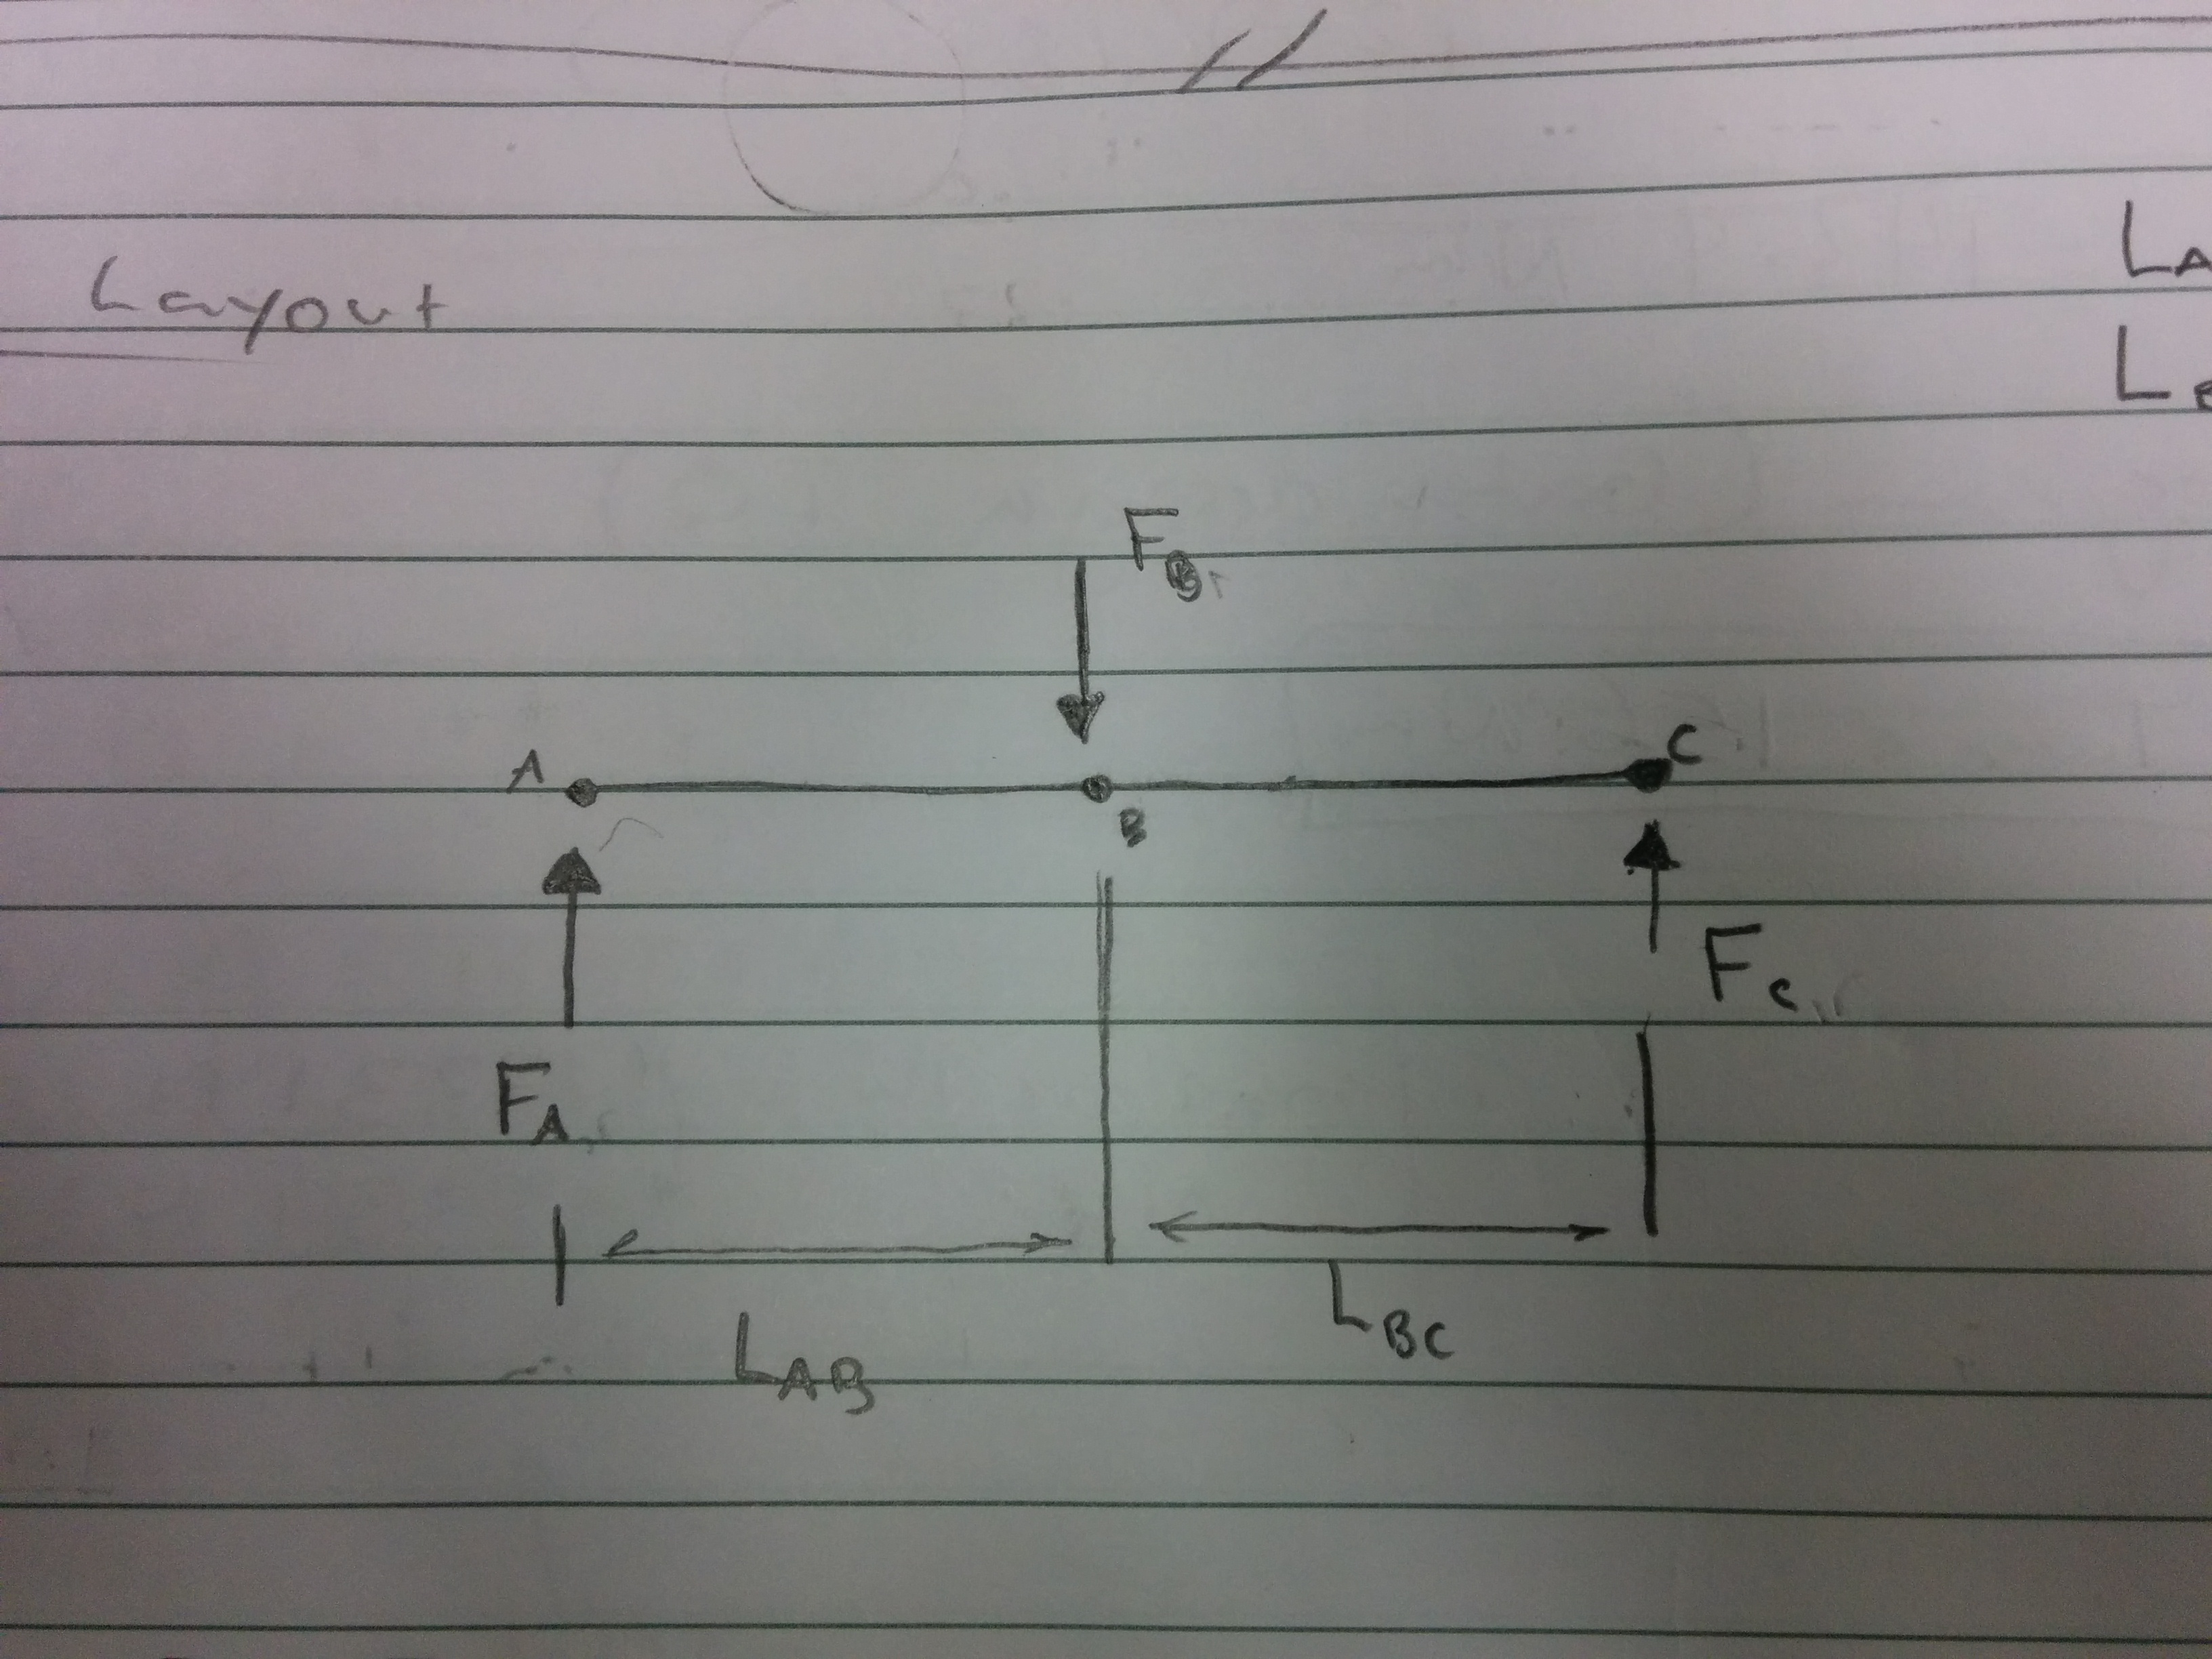
\includegraphics[width=\linewidth]{images/fb_output_shaft.jpg}
	\caption{Free Body Diagram for Output Shaft.}
	\label{fig:fb_output_shaft}
\end{figure}
\begin{table}[H]
	\centering
	\caption{Output Shaft Design Specifications}
	\begin{tabular}{| p{5cm}llp{7cm} |} \hline
		Requirement & Value & Unit & Reason \\ \hline
		Torque Transmission & 156 & Nm & Max torque transmitted by motor to the driveshaft assuming operation at 895.2\,W through a 30:1 reduction \\
		Radial Load & 3331	& N & Radial load applied by drive sprocket \\ \hline
	\end{tabular}
	\label{tab:output_shaft_specs}
\end{table}


\section{Drive Box Assembly}

The drive box is an aluminum structure build to house the external belt drive system. It consists of four separate aluminum plates bolted together around the perimeter for modular assembly. Three of the plates are structural, while the fourth frontmost plate serves only a sealing purpose. There are five separate bearing housings protruding from the drive box and bolted to the structural plates: three in the front (the wheel shaft passes through two of them), and two in the back. The pivot is bolted through the back plate. The drive box is shown in Figures~\ref{fig:box_bld} and~\ref{fig:box_in}. Buna-N o-rings are installed between each separate component of the drive box to ensure proper sealing.

\begin{figure}[htbp]
\centering
\begin{minipage}{0.45\linewidth} \centering
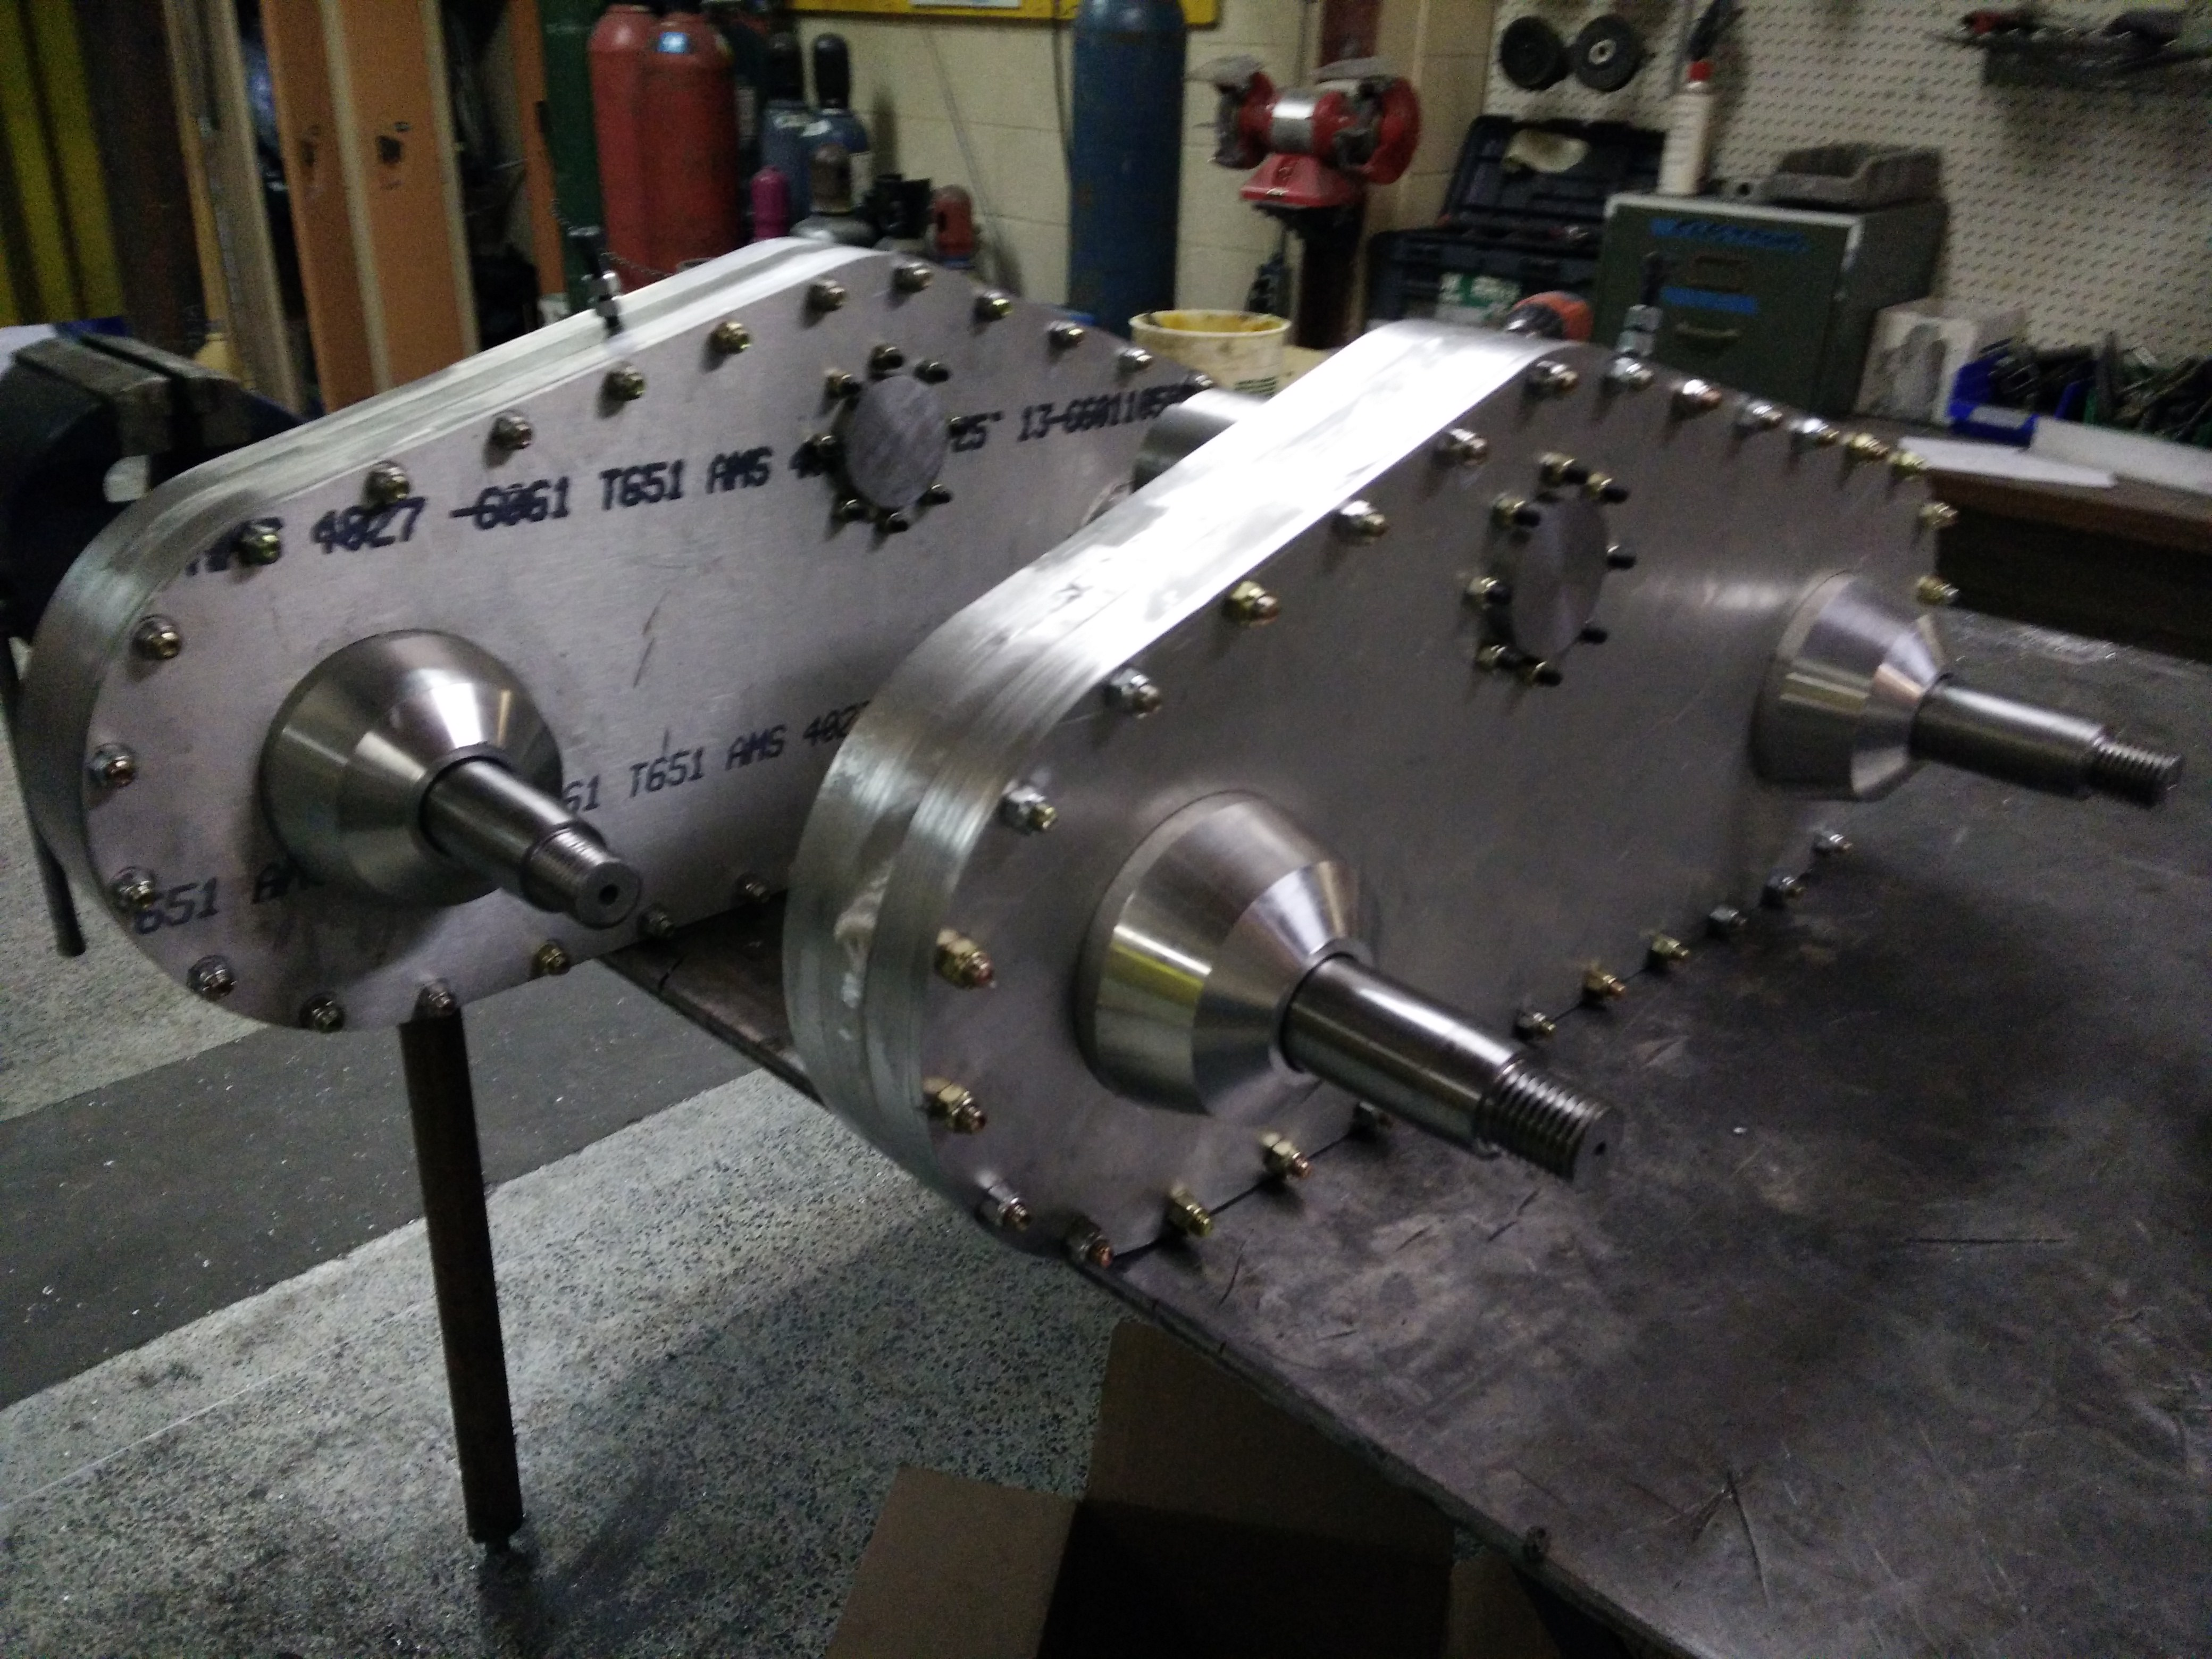
\includegraphics[height=0.22\textheight]{images/drive_box_assembly_NEW_bld}
\captionof{figure}[Completed Drive Boxes]{Two completed drive boxes before being mounted on the robot. One is the mirror image of the other.}
\label{fig:box_bld}
\end{minipage}
\hfill
\begin{minipage}{0.45\linewidth}
\centering
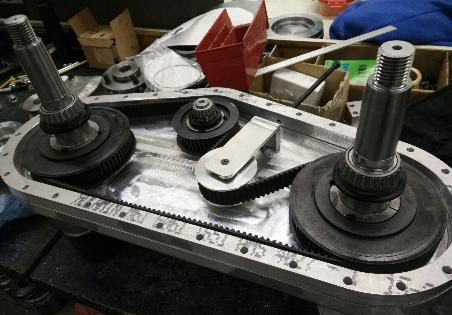
\includegraphics[height=0.22\textheight]{images/drive_box_open_bld}
\captionof{figure}[Interior of the Drive Boxes]{The drive box houses two wheel shaft assemblies, one drive shaft assembly, the belt, and tensioner.}
\label{fig:box_in}
\end{minipage}
\end{figure}

\subsection{Design Constraints}

The main constraints imposed on the drive box design are dimensional since the drive box design is constrained by the components in houses. It houses the belts, sprockets, bearing, seals, and tensioner. These components must also be laid out as defined by the shaft design software as presented in Section~\ref{SECTION LABEL FOR SHAFT}. %% TODO
Drive box dimension constraints are summarized in Table~\ref{tab:box_dim}. The drive box must be large enough to fit all the components, with additional clearance around the belt and sprocket for installation ease.

\begin{table}[htbp]
\centering
\caption{Gearbox dimension constraints}
\begin{tabular}{| lll |}\hline
Component & Dimension & Value \\ \hline
\multirow{2}{*}{Driving sprocket} & Diameter & 5  in \\
& Width & over 1.5 in \\
\multirow{2}{*}{Wheel sprocket} & Diameter & 7.6  in \\
& Width & over 1.5 in \\ \hline
\end{tabular}
\label{tab:box_dim}
\end{table}

\subsection{Functional Requirements}

The drive boxes serve two main purposes: house the interior components from the environment and support the weight of the robot with negligible deflection. Therefore, the drive box must be adequately sealed to prevent entry of fluids and/or dust particles that can cause belts to slip. They must also be strong enough not to deflect under the weight of the robot, or under the high forces seen during skid steers. This requirement is important for the obvious reason, but it is of particular importance for a belt drive. Sprockets must not lie out of plane, as this puts point loads on the belt and decrease its life.

\subsection{Analysis and Design}
\section{Battery Rack}

\subsection{Design Constraints}
\subsection{Functional Requirements}
\subsection{Analysis and Design}
\subsubsection{Battery Mounts}
\subsubsection{Battery Support Frame}

\section{Frame Assembly}
The full frame and chassis of the vehicle were provided, however some modifications were necessary in order to incorporate the new design which allowed the 30:1 reduction box output shaft be coupled to the drive shaft of the drive box using a flexible coupling. In addition to the horizontal cross member, four vertical members were placed on the corners of the horizontal crossers to direct forces up through the rest of the frame, thus reducing the reliance on the welds to hold the weight of the vehicle. Furthermore, aluminum inserts were welded to the frame hole cutouts, in which brass bushings were pressed. The aluminum insert had a tapped hole with a grease nipple and a shoulder to separate both brass bushings, allowing grease to be put between the pivot and bushings. The frame assembly can be seen in Figure \ref{fig:battery_rack_and_frame_mount_drw}, and highlights both the horizontal and vertical supports. 

In order to accomodate the design allowing for the 30:1 worm gear reduction box output shaft to be coupled to the drive shaft of the drive box, the output hole in the frame needed to be raised by 10\,cm. The existing frame base member was 2x2x1/8'' rectangular tubing, however to increase the output hole height it was required that 2x8x3/16'' rectangular tubing was used. 

\begin{figure}[h]
\centering
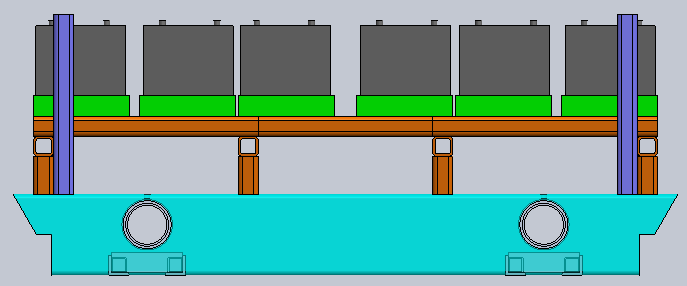
\includegraphics[width=0.7\linewidth]{./images/battery_rack_and_frame_mount_drw}
\caption{Frame Assembly Including Battery Rack and Frame Extension}
\label{fig:battery_rack_and_frame_mount_drw}
\end{figure}
 
\subsection{Design Constraints}
The design of the frame insert was constrained by the length of the vehicle, and needed to be made out rectangular tubing high enough to accomodate the output hole for the pivot. Since the frame shell could not be removed, the frame insert needed to be custom made to fit into the space where the old horizontal members were cut out. Many attempts were made at modelling the modifications, however the greatest success came from creating a cardboard template from which the desired geometry was finally cut out of the tubing. The vertical supports would need to rest on top of the rectangular tubing and extend into the top portion of the frame. The entire addition needed to be made out of the same grade of aluminum as the frame was to be weldable. 
\subsection{Functional Requirements}

\subsection{Analysis and Design}
\subsubsection{Frame}
\subsubsection{Aluminum Insert}
\subsubsection{Bushings}